\documentclass{beamer}
\usepackage[utf8]{inputenc}
\usepackage[english]{babel}
\usepackage{csquotes, amsmath,amsfonts,amssymb, amsthm, svg}

\newcommand{\nologo}{\setbeamertemplate{logo}{}}
\newcommand{\noframenumber}{\setbeamertemplate{navigation symbols}{}}

\usetheme{moloch}
\setbeamercolor{block body}{bg=mDarkTeal!30}
\setbeamercolor{block title}{bg=mDarkTeal, fg=black!2}
\setbeamercolor{background canvas}{bg=white}

\newtheorem{hypothesis}{Hypothesis}

\newcommand\blfootnote[1]{%
  \begingroup
  \renewcommand\thefootnote{}%
  \renewcommand\footnotemark{}%
  \footnotetext{#1}
  \addtocounter{footnote}{-1}%
  \endgroup
}

\title{Error bounds for non-smooth right-hand sides}
\author{\underline{Felix Mest}, Martin Arnold}
\institute{felix.mest@mathematik.uni-halle.de\\Martin-Luther-University Halle-Wittenberg \\ Institute of Mathematics}
\logo{\includegraphics[height=1cm]{../../../uhallelogo.png}}

\begin{document}

\frame{\titlepage}

{
\nologo
\begin{frame}{Problem statement}
  \onslide<1->{

  Find error bounds for the numerical integration of
  \[
    y_{s}'(t) = f(t, y_{s}(t), s(t, y_{s}(t))),\quad (t\in [t_{0}, t_{e}]), \quad y_{s}(t_{0}) = y_{0},
  \]
  where $s$ is \enquote{reasonably non-smooth}.
  }
  \onslide<2->{
  \begin{definition}
    A function $s$ is reasonably non-smooth, if 
    \begin{enumerate}
      \item $s \in C^{k}, k\in \mathbb{N}_{0}$,
      \item $s^{(k+1)}$ discontinuous only at finitely many points and
      \item $s$ has uniformly bounded (weak) derivatives up to order $k+1$, i.e. given $L > 0,\,\lVert s^{(r)} \rVert_{\infty} \leq L,\, r = 0, 1, \dots, k + 1$.
    \end{enumerate}
  \end{definition}
  }
\end{frame}
}

\begin{frame}{Application}
  \begin{itemize}
    \item Real-world data for $u$ in the smooth system 
    \[
      y_{u}'(t) = f(t, y_{u}(t), u(t, y_{u}(t))),\quad (t\in [t_{0}, t_{e}]), \quad y_{u}(t_{0}) = y_{0}
    \]
    known only at finitely many times
    \item Real-world data available for $y$, but (potentially non-smooth) dynamics unknown (NeuralODE)
    \item Physical model is non-smooth (impact, switches, different time scales)
  \end{itemize}
\end{frame}

{
\nologo
\begin{frame}{Towards error estimates, Arnold 2010}
  \begin{theorem}
    The numerical integration of
    \[
      y_{s}'(t) = f(t, y_{s}(t), s(t)), \quad (t\in [t_{0}, t_{e}]), \quad y_{s}(t_{0}) = y_{0},
    \]
    where $s\in C^{k}, (k = 0, 2),$ is a linear or cubic spline of $u(t)$, yields local error estimates
    \[
      \lVert le_{n} \rVert = \mathcal{O} (h^{p+1}) \text{ and } \lVert le_{n} \rVert = \mathcal{O} (h^{p+1}) + \mathcal{O}(h^{k+2}).
    \]
    and since $s^{(k+1)}$ discontinuous only at finitely many points the global error estimate
    \[
      \lVert e_{n} \rVert = \mathcal{O} (h^{p}) + \mathcal{O} (h^{k+2}). 
    \]
  \end{theorem}
\end{frame}
}

\begin{frame}{Excited Oscillator, 5th order RK, linear spline}
  $y_{1}''(t) + y_{1}(t) = u(t),\, u(t) = \alpha\sin(\omega t), y_{2} = y_{1}'$.
  \includesvg[width=\textwidth, height = .5\textheight]{images/splinef1.svg}
  $y_{1}(0) = 1,\, y_{1}'(0) = 0,\, y_{1}' = y_{2}, \alpha = 0.5, \omega = 0.3, t_{0} = 0, t_{e} = 10$.
\end{frame}

\begin{frame}{Excited Oscillator, 5th order RK, step width control}
  $y_{1}''(t) + y_{1}(t) = u(t),\, u(t) = \alpha\sin(\omega t), y_{2} = y_{1}'$.
  \includesvg[width=\textwidth, height = .5\textheight]{images/splineffixed1.svg}
  $y_{1}(0) = 1,\, y_{1}'(0) = 0,\, y_{1}' = y_{2}, \alpha = 0.5, \omega = 0.3, t_{0} = 0, t_{e} = 10$.
\end{frame}

\begin{frame}{Excited Oscillator, 7th order RK, cubic spline}
  $y_{1}''(t) + y_{1}(t) = u(t),\, u(t) = \alpha\sin(\omega t), y_{2} = y_{1}'$.
  \includesvg[width=\textwidth, height = .5\textheight]{images/splinef3.svg}
  $y_{1}(0) = 1,\, y_{1}'(0) = 0,\, y_{1}' = y_{2}, \alpha = 0.5, \omega = 1, t_{0} = 0, t_{e} = 10$.
\end{frame}

\begin{frame}{Proof sketch (1/3)}
  \includesvg[width=\textwidth, height = .5\textheight]{images/leftright.svg}
  \begin{itemize}
    \item<1-> Assume single discontinuity $\tau$ in step $t_{n} \to t_{n+1}$
    \item<2-> Left and right Taylor polynomials $s^{-}(t), s^{+}(t)$ around $\tau$
    \item<3-> Continue each on $[t_{n}, t_{n+1}]$
    \item<4-> $\lVert s^{+}(t) - s^{-}(t) \rVert \leq 2Lh^{k+1} / ((k+1)!)$
  \end{itemize}
\end{frame}

{
  \nologo
  \begin{frame}{Proof sketch (2/3)}
    \includesvg[width=\textwidth, height = .5\textheight]{images/leftrightsmooth.svg}
    \begin{itemize}
    \item<1-> Define smoothed system input $\tilde{s}(t) = (1-\lambda)s^{-}(t) + \lambda s^{+}(t), \quad \lambda = (t-t_{n}) / (t_{n+1} - t_{n})$
    \item<2-> $\lVert \tilde{s}(t) - s(t) \rVert \leq 2Lh^{k+1} / ((k+1)!) $
    \item<3-> Local, smooth shadow problem $\bar{y}_{\tilde{s}}'(t) = f(t, \bar{y}_{\tilde{s}}(t), \tilde{s}(t)), \bar{y}(t_{n}) = y(t_{n})$
    \item<4-> $\lVert \bar{y}_{\tilde{s}}(t) - y_{s}(t) \rVert \leq C_{0} (e^{L_{f, s}h} - 1)h^{k+1} \leq Ch^{k+2}$ (asymptotically)
  \end{itemize}
\end{frame}
}

\begin{frame}{Proof sketch (3/3)}
  Result ($t_{n} \to t_{n+1}, \tau \in [t_{n}, t_{n+1}]$):
  \begin{align*}
    \lVert le_{n} \rVert &= \lVert \textcolor{red}{y_{s}(t_{n+1})} - \textcolor{cyan}{(y_{s}(t_{n}) + h\Phi(y_{s}(t_{n}); h, f, s))} \rVert \\
    &= \lVert \textcolor{red}{y_{s}(t_{n+1})} \\
    &- \textcolor{blue}{\left( y_{s}(t_{n}) + h\Phi(y_{s}(t_{n}); h, f, \tilde{s})\right)}\\
    &+\textcolor{cyan}{\left( y_{s}(t_{n}) + h\Phi(y_{s}(t_{n}); h, f, \tilde{s})\right)}\\
    &\textcolor{red}{-\bar{y}_{\tilde{s}}(t_{n+1})}\\
    &+\textcolor{blue}{\bar{y}_{\tilde{s}}(t_{n+1})}\\
    &\textcolor{cyan}{-\left( y_{s}(t_{n}) + h\Phi(y_{s}(t_{n}); h, f, s)\right)} \rVert \\
    &\leq \textcolor{red}{Ch^{k+2}} + \textcolor{blue}{\mathcal{O}(h^{p+1})} + \textcolor{cyan}{L_{\Phi, s}h^{k+2}} \\
    &= \mathcal{O} (h^{p+1}) + \mathcal{O} (h^{k+2}).
  \end{align*}

\end{frame}


%\begin{frame}{Excited Oscillator, 4th order RK, $s$ piecewise constant}
%  $y_{1}''(t) + y_{1}(t) = u(t),\, u(t) = \alpha\sin(\omega t)$.
%  \includesvg[width=\textwidth, height = .5\textheight]{images/splinef0.svg}
%  $y_{1}(0) = 1,\, y_{1}'(0) = 0,\, y_{1}' = y_{2}, \alpha = 0.1, \omega = 0.1, t_{0} = 0, t_{e} = 10$.
%\end{frame}

\begin{frame}{Excited Oscillator, 4th order RK, ReLU network $s$}
  $y_{1}''(t) + y_{1}(t) = u(t),\, u(t) = \alpha\sin(\omega t)$.
  \includesvg[width=\textwidth, height = .5\textheight]{images/relus.svg}
  $y_{1}(0) = 1,\, y_{1}'(0) = 0,\, y_{1}' = y_{2}, \alpha = 0.5, \omega = 0.3, t_{0} = 0, t_{e} = 10$.
\end{frame}

\begin{frame}{Excited Oscillator, 4th order RK, Fourier $s$}
  $y_{1}''(t) + y_{1}(t) = u(t),\, u(t) = \alpha\sin(\omega t)$.
  \includesvg[width=\textwidth, height = .5\textheight]{images/fourier.svg}
  $y_{1}(0) = 1,\, y_{1}'(0) = 0,\, y_{1}' = y_{2}, \alpha = 1, \omega = 1, t_{0} = 0, t_{e} = 10$.
\end{frame}
{
\nologo
\begin{frame}{Generalization of previous theorem}
  \begin{theorem}
    The numerical integration of
    \[
      y'(t) = f(t, y(t), s(t)), \quad y(t_{0}) = y_{0},
    \]
    where $s$ is reasonably non-smooth yields local error estimates
    \[
      \lVert le_{n} \rVert = \mathcal{O} (h^{p+1}) \text{ and } \lVert le_{n} \rVert = \mathcal{O} (h^{p+1}) + \mathcal{O}(h^{k+2}).
    \]
    and as before
    \[
      \lVert e_{n} \rVert = \mathcal{O} (h^{p}) + \mathcal{O} (h^{k+2}). 
    \]
  \end{theorem}
\end{frame}
}

%{
%\nologo
%\begin{frame}{Refined error bound (1/2)}
%  \begin{theorem}
%    The numerical integration of
%    \[
%      y'(t) = f(t, y(t), s(t)), \quad y(t_{0}) = y_{0},
%    \]
%    where $s$ is reasonably non-smooth yields
%    \[
%      \lVert e_{n} \rVert \leq \min_{r\leq \tilde{p}}\{C_{r}h^{r}\} + \mathcal{O}(h^{k+2}),
%    \]
%    where $C_{r}$ are constants dependent on derivatives of $y$ and $\tilde{p} = \min\{p, k\}$
%  \end{theorem}
%\end{frame}
%}
%
{
\nologo
\begin{frame}{Refined error bound}
  A \enquote{NeuralODE} (NeuralQuadrature) for solving Euler's elastica using $3$-point Gaussian quadrature.
  \[
  \displaystyle \left|\int_{a}^{b}f(x)dx - \hat{\mathrm{I}}(f;a,b,h)\right| \leq \min_{r\leq k}\{C_{r}\lVert  f^{(r)}\rVert_{\infty}\,h^{r}\}
  \]
  \includesvg[width=\textwidth]{images/refinederrorbound.svg}
  \blfootnote{Celledoni, E.; Cokaj, E.; Leone, A.; Leyendecker, S.; Murari, D.; Owren, B.; Sato Martin de Almagro, R.; Stavole, M. (2024): Neural networks for the approximation of Euler’s elastica”. CMAME 435.117584.}
\end{frame}
}

%\begin{frame}{Excited Oscillator, 4th order RK, Tanh $s$}
%  $y_{1}''(t) + y_{1}(t) = u(t),\, u(t) = \sin(t),\, y_{1}(0) = 1,\, y_{1}'(0) = 0,\, y_{1}' = y_{2}$.
%  \includesvg[width=\textwidth, height = .5\textheight]{images/tanhs.svg}
%\end{frame}
{
\nologo
\begin{frame}{State-dependent system input}
  Rotating machinery, torsional dynamics:
  \begin{itemize}
    \item Lathe with uneven workpiece
    \item Drilling anisotropic rocks (oil and gas exploration) 
    \item Rub-impact rotors
  \end{itemize}
  \blfootnote{Liu, X; Hou, X:, Meng, G. (2026): Dynamics of a nonlinear oscillator with space-time phase-modulated excitation. International Journal of Non-Linear Mechanics, 187.}

\end{frame}

\begin{frame}{State-dependent system input}
  \begin{minipage}{0.6\textwidth}
    $my_{1}''(t)+\alpha y_{1}(t) + \gamma y_{1}'(t) = u(t, y_{1}(t))$
  \end{minipage}
  \begin{minipage}{0.3\textwidth}
    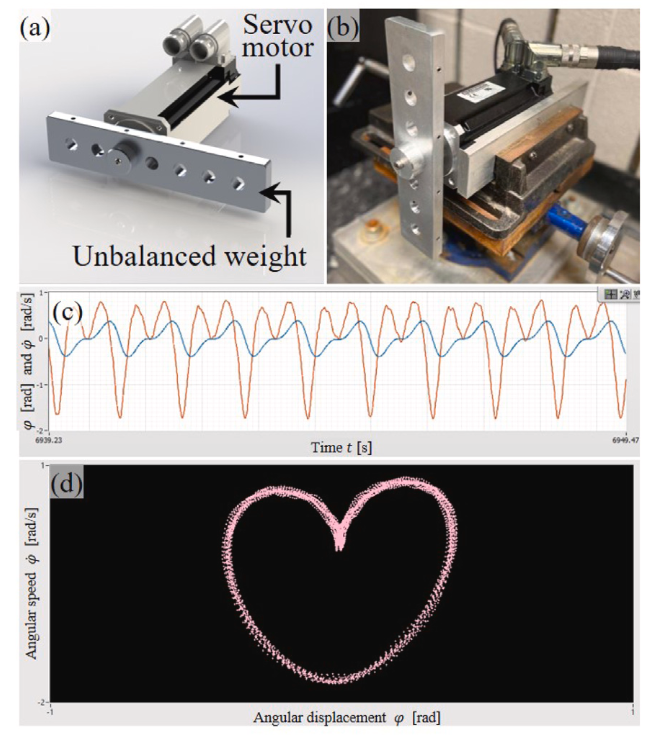
\includegraphics[height=.6\textheight]{images/unbalanced.png}
  \end{minipage}
  \blfootnote{Liu, X; Hou, X:, Meng, G. (2026): Dynamics of a nonlinear oscillator with space-time phase-modulated excitation. International Journal of Non-Linear Mechanics, 187.}
\end{frame}

}

\begin{frame}{State-dependent system input, linear spline}
  $y_{1}''(t) + \alpha y_{1}(t) + \gamma y_{1}'(t) = \beta \sin(\omega t + \kappa y_{1}(t))$ 
  \includesvg[width=\textwidth, height = .5\textheight]{images/statesplinef1.svg}
  $\alpha = 1.104, \beta = 3, \gamma = 0.958, \omega = 0.1, \kappa = 1, t_{0} = 0, t_{e} = 10$.
\end{frame}

\begin{frame}{State-dependent system input, cubic spline}
  $y_{1}''(t) + \alpha y_{1}(t) + \gamma y_{1}'(t) = \sin(\omega t + \kappa y_{1}(t))$ 
  \includesvg[width=\textwidth, height = .5\textheight]{images/statesplinef3.svg}
  $\alpha = 1.104, \beta = 3, \gamma = 0.958, \omega = 0.1, \kappa = 1, t_{0} = 0, t_{e} = 10$.
\end{frame}

{
\nologo
\begin{frame}{Natural hypothesis}
  \begin{hypothesis}
    The numerical integration of
    \[
      y'(t) = f(t, y(t), s(y(t))), \quad y(t_{0}) = y_{0},
    \]
    where $s$ is reasonably non-smooth yields local error estimates
    \[
      \lVert le_{n} \rVert = \mathcal{O} (h^{p+1}) \text{ and } \lVert le_{n} \rVert = \mathcal{O} (h^{p+1}) + \mathcal{O}(h^{k+2}).
    \]
    and as before the global error estimate
    \[
      \lVert e_{n} \rVert = \mathcal{O} (h^{p}) + \mathcal{O} (h^{k+2}). 
    \]
  \end{hypothesis}
\end{frame}
}

\begin{frame}{Proof Sketch}
  Different to before:
  \begin{itemize}
    \item Assume $[t_{n}, t_{n+1}]$ contains at most one $\tau _{i}$, such that $s(y(\tau_{i}))$ discontinuous (quite restricting)
    \item Left and right Taylor polynomials
    \begin{align*}
      s^{-}(y(t)) &= s(y(\tau_{i})) + (t-\tau_{i}) s_{y}(y(\tau_{i}))f(y(\tau_{i}), s(y(\tau_{i}))) + \dots,\\
      s^{+}(y(t)) &= s(y(\tau_{i})) + (t-\tau_{i}) s_{y}(y(\tau_{i}))f(y(\tau_{i}), s(y(\tau_{i}))) + \dots,
    \end{align*}
    $\to$ bound on $\frac{d^{k+1}}{dt^{k+1}}s(y(t))$ \\
    $\to$ generalized elementary differentials
  \end{itemize}
\end{frame}

\begin{frame}{Example: Corresponding Trees of order $4$}
  \includesvg[height=.3\textheight]{images/graphviz.svg}
  \includesvg[height=.4\textheight]{images/graphviz(1).svg}
\end{frame}
\begin{frame}{Unavoidable multiplicity of discontinuities in step $t_{n} \to t_{n+1}$}
  \vspace*{-1cm}
  Finitely many $\to$ Similiar result, growing error constants\\
  Infinitely many $\to$ Equilibria or infinite oscillations in finite time
  $\to$ Loss of one order?
  \includesvg[width=\textwidth, height = .5\textheight]{images/infoscill.svg} 
  $y_{1}'' + \mathrm{sign}(y_{1}) \sqrt{\lvert y_{1} \rvert } + 0.5 y_{2} = 0,\, y_{1}(0) = 1,\, y_{2}'(0) = 0, y_{2} = y_{1}'$.
\end{frame}

\begin{frame}{Conclusion}
  \begin{itemize}
    \item Error bounds for spline $s = s(t)$ directly transferable to other reasonably non-smooth $s = s(t)$
    \item Refined error bound useful in oscillatory context
    \item Also transferable to state-dependent $s = s(y(t))$, but with more restrictive assumptions
    \item Experimentally, without assumptions, loss of one order seems to be the case, but more work needed
  \end{itemize}
\end{frame}
\end{document}